\section{Versuchsaufbau/-durchführung}
Der verwendete Aufbau, der in allen Teilen der Durchführung nur geringfühgig modifiziert wird, ist in
Abbidung \ref{fig: aufbau} schematisch dargestellt. Mit einem Heizgenerator kann die Temperatur im Gehäuse
eingestellt und mit einem elektrischen Thermometer gemessen werden. Sowohl die Spannungsquelle für die
Beschleunigungsspannung $U\ua{B}$ als auch jene für die Abbremsspannung $U\ua{A}$ verfügt über
eine zeitlich gesteuerte Regelung. Die Auffängeranode ist über eine abgeschirmte Leitung, die
äußere Einflüsse minimieren soll, mit dem $Y$-Eingang eines $XY$-Schreibers verbunden. Je nach Teil der
Durchführung wird entweder $U\ua{B}$ oder $U\ua{A}$ an die $X$-Achse angelegt. Der Aufbau ermöglicht somit
eine Aufzeichnung der Kurven $I\ua{A}(U\ua{B})$ ($I\ua{A}$ gegen $U\ua{B}$) bzw. $I\ua{A}(U\ua{A})$ ($I\ua{A}$ gegen $U\ua{A}$).
\begin{figure}[H]
  \centering
  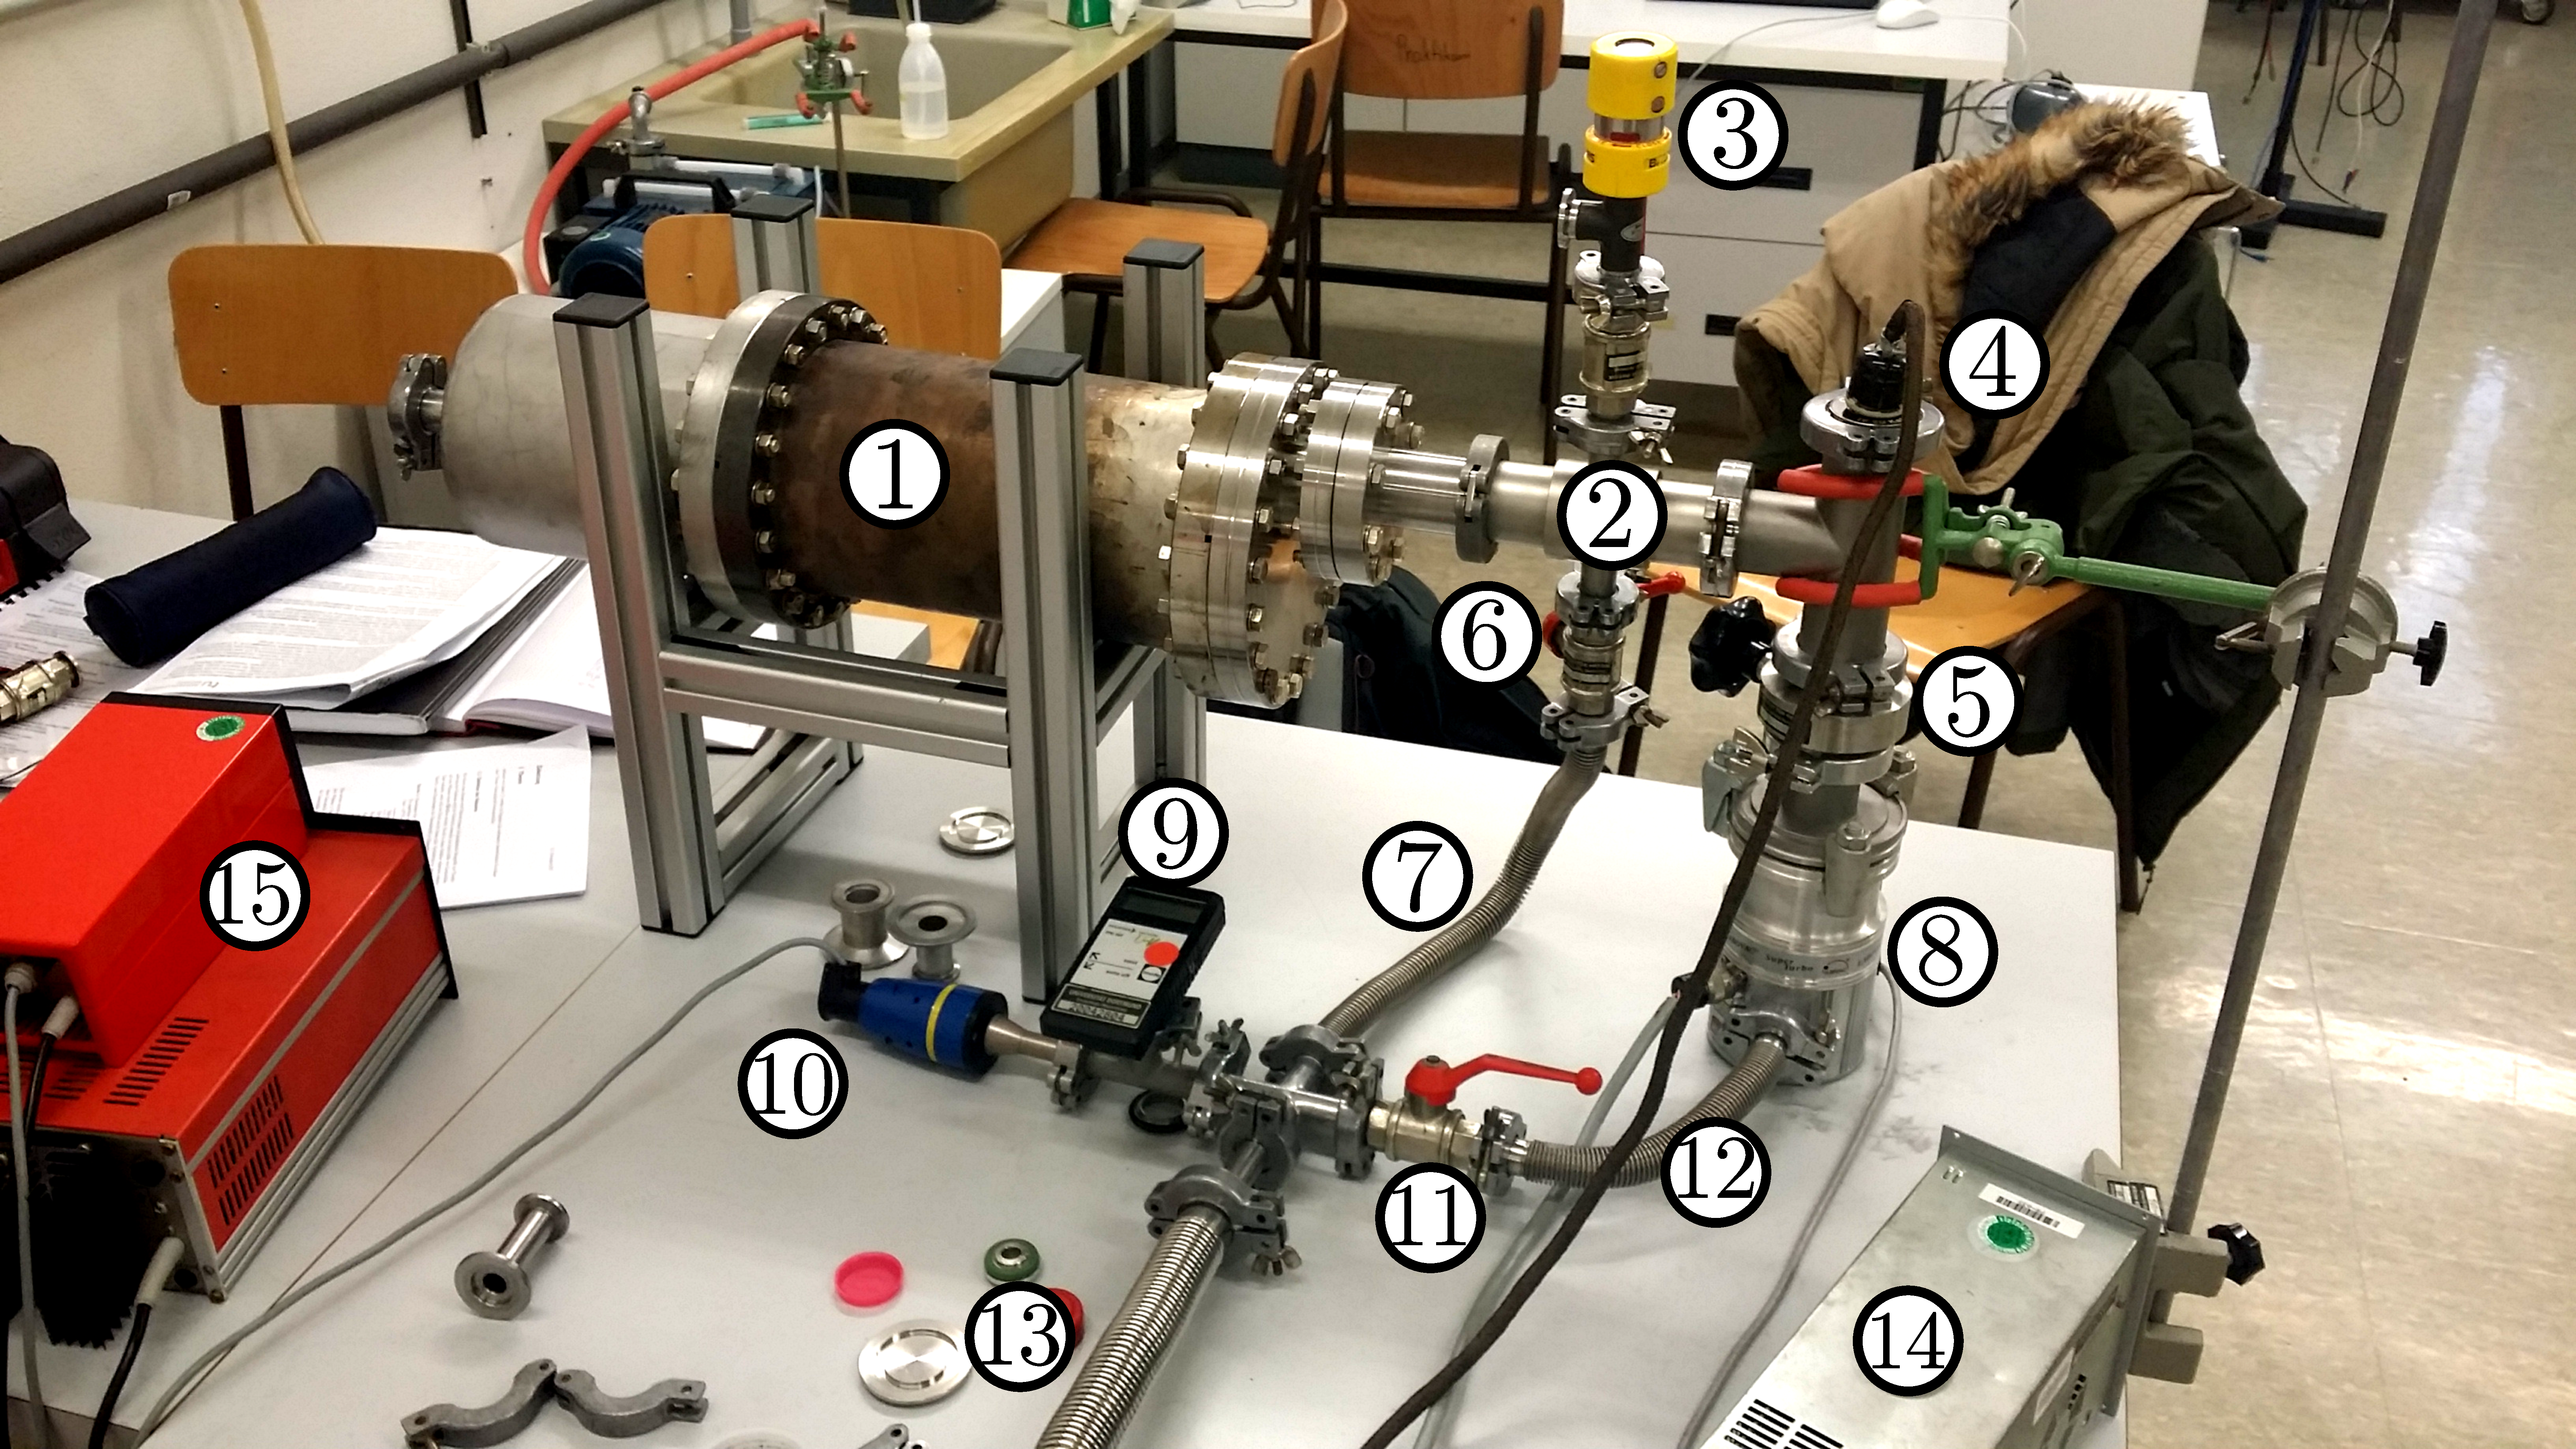
\includegraphics[width = 0.8\textwidth]{pics/aufbau.png}
  \caption{Schematische Darstellung des Aufbaus zur Durchführung des Franck-Hertz-Versuches \cite{anleitung601}.}
  \label{fig: aufbau}
\end{figure}

\subsection{Qualitative Untersuchung des Energiespektrums}
Für diesen Aufgabenteil wird die Bremsspannung $U\ua{A}$ mit dem $X$-Eingang des Schreibers verbunden. Die
Beschleuingungsspannung $U\ua{B}$ wird auf den konstanten Wert $\SI{11}{\volt}$ eingestellt.
Wie bereits
in der Therie erwähnt stellt der Anodenstrom $I\ua{A}$ ein Maß für die Anzahl derjeniger Elektronen dar, deren %Theorie
kinetische Energie die Ungleichung \eqref{eq: ungl_E_kin} erfüllen.
Unter variabler Spannung $U\ua{A}$ wird daher der Anodenstrom $I\ua{A}$ mit dem $XY$-Schreiber aufgezeichnet.
Mit der zeitlichen Reglung der Spannungsquelle wird die Spannung mit einer mittleren Geschwindigkeit von etwa
$\SI{0.3}{\volt \per\second}$ von $\SI{0}{\volt}$ auf $\SI{10}{\volt}$ hochgeregelt. Die erhaltene Kurve ermöglicht
qualitative Aussagen über die integrale Energieverteilung der mit $U\ua{B}$ beschleunigten Elektronen.
Die differentielle Energieverteilung lässt sich ermitteln, indem für ein kleines Spannungsintervall
$\Delta U\ua{A}$ $I(U\ua{A}) - I(U\ua{A} + \Delta U\ua{A})$ gegen $U\ua{A}$ aufgetragen wird. Das Maximum
der so ermittelten Kurve ist um $K$ von $U\ua{B}$ verschoben. Die Untersuchung der Kurve ermöglicht somit eine
erste Bestimmung des Wertes für $K$.
Der Prozess wird unter Raumtemperatur und $T \approx \SI{150}{\celsius}$ untersucht.

\subsection{Aufzeichnung der Franck-Hertz-Kurve}
Zur experimentellen Bestimmung der Anregungsenergie des \ce{Hg}-Atoms wird die Franck-Hertz-Kurve für
verschiedene Temperaturen (zwischen $\num{160}$ und $\SI{200}{\celsius}$) aufgezeichnet.
Die Bremsspannung wird auf den konstanten Wert $U\ua{A} = \SI{1}{\volt}$ eingestellt.
Die Beschleuinigungsspannungg wird an den $X$-Eingang des Schreibers gelegt und zwischen $\SI{0}{\volt}$
und $\SI{55}{\volt}$ mit einer Geschwindigkeit von etwa $\SI{2}{\volt \per\second}$ erhöht. Für die
Auswertung wird eine Kurve mit möglichst vielen ausgeprägten Maxima gewählt. Neben der Anregungsenergie,
die sich gemäß \ref{eq: anregungsenergie} mit dem Abszissenabstand $U\ua{1}$ zwischen den Strommaxima ergibt,
kann eine weitere Messung der Verschiebung
$K$ durchgeführt werden. Das $n$-te Maximum befindet sich im Abstand $d\ua{U}$ vom Ursprung.
\begin{equation}
  d\ua{U} = nU\ua{1} + K \quad \Leftrightarrow \quad K = d\ua{U}- n U\ua{1}.
  \label{eq: k_franck}
\end{equation}

\subsection{Bestimmung der Ionisierungsspannung von \ce{Hg}}
Als Ionisierungsspannung $U\ua{ion}$ bezeichnet man jene Spannung, mit der ein Elektron beschleunigt werden
muss, sodass es beim elastischen Stoß ein Atom ionisieren kann. Bei diesem Versuchsteil sollen die bei diesem
Prozess entstehenden positiven Ionen nachgewiesen werden. Hierzu wird die Abbremsspannung in umgekehrter Polung
auf $\SI{-30}{\volt}$ eingestellt und der Strom $I\ua{A}$ in Abhängigkeit von der Beschleunigungsspannung $U\ua{B}$
mit dem $XY$-Schreiber gemessen. Hierzu wird $U\ua{B}$ an den $X$-Schreiber angeschlossen und die Spannung mit einer %X-Eingang des XY-Schreibers
mittleren Geschwindigkeit von ca. $\SI{2}{\volt \per\second}$ zwischen $\SI{0}{\volt}$ und $\SI{50}{\volt}$ hochgeregelt.
Der so ermittelte Graph ermöglicht unter Berücksichtigung der Verschiebung \ref{eq: effektivspannung} eine
experimentelle Bestimmung der Ionisationspannung $U\ua{ion}$. Der Versuchteil wird bei einer Temperatur von etwa $\SI{100}{\celsius}$
durchgeführt.
